\documentclass[conference]{IEEEtran}

\usepackage[utf8]{inputenc}
\usepackage[T1]{fontenc}
\usepackage{cite}
\usepackage{amsmath}
\usepackage{booktabs}
\usepackage{array}
\usepackage{url}
\usepackage{graphicx}
\usepackage{balance}

\title{Student Dropout Prediction Using Machine Learning}

\author{
\IEEEauthorblockN{Henrique Reveles, n.\textordmasculine{} 119786\\
Gonçalo Simões, n.\textordmasculine{} 119412\\
Geovanni Santos, n.\textordmasculine{} 115637}
\IEEEauthorblockA{
Introdução à Aprendizagem Automática\\
Universidade de Aveiro}
}

\begin{document}
\maketitle

\begin{abstract}
University dropout is not only a number in an institutional dashboard; it is often the visible end of a longer process of academic difficulty, financial pressure and loss of belonging. Recent European and OECD evidence shows the scale of the challenge: across the EU25, 13.4\% of bachelor's students leave their programme during the first year, and across OECD countries only 43\% of students who start a bachelor's programme complete a tertiary degree within the theoretical duration. In this context, early and responsible identification of students at risk can help institutions act before disengagement becomes irreversible. This work studies supervised machine learning for academic dropout prediction using 4424 student records and 34 demographic, socioeconomic, administrative and academic input variables. The main formulation is binary classification, distinguishing \textit{Dropout} from \textit{Non-Dropout}, with an additional multiclass experiment over \textit{Dropout}, \textit{Enrolled} and \textit{Graduate}. Five models were compared using stratified cross-validation: Logistic Regression, Random Forest, AdaBoost, Gradient Boosting and Hist Gradient Boosting. The best final binary model was Gradient Boosting, reaching 87.57\% accuracy on the test set, with 79.17\% F1-score and 73.59\% recall for the \textit{Dropout} class. The final confusion matrix shows 209 correctly detected dropout cases and 75 missed dropout cases. These results are promising, but they also make the ethical boundary clear: the model can support human early-warning decisions, not replace them.
\end{abstract}

\begin{IEEEkeywords}
student dropout, machine learning, classification, educational data mining, early warning systems, gradient boosting
\end{IEEEkeywords}

\section{Introduction}
Student dropout prediction is a supervised learning problem with practical relevance for higher education institutions. Dropout is costly for students, families and public education systems, and it often reflects difficulties that accumulate over time rather than a single isolated event. European Commission monitoring reports indicate that, across the EU25, 13.4\% of bachelor's students leave their programme during the first year \cite{ec2025monitor}. Eurostat also reports that 14.2\% of people aged 15--34 in the EU had left formal education or training at least once during their lifetime, based on 2024 data \cite{eurostat2025dropout}. From a completion perspective, the OECD reports that only 43\% of students entering bachelor's programmes complete a tertiary degree within the theoretical duration, although completion increases when longer time windows are considered \cite{oecd2025completion}. These numbers show that dropout is not a marginal phenomenon; it is a structural challenge for higher education.

If students at risk of abandoning their studies can be identified early, academic services may provide tutoring, financial guidance or pedagogical support before the situation becomes irreversible. However, this problem is complex because dropout is influenced by academic performance, socioeconomic conditions, administrative constraints and personal factors that are only partially represented in institutional data.

The goal of this project is to build and evaluate machine learning models capable of predicting dropout risk from structured student data. The complete project repository, including the notebook, report files, dataset and generated figures, is available online \cite{github2026project}. The original target has three possible values: \textit{Dropout}, \textit{Enrolled} and \textit{Graduate}. Since the most direct practical objective is to detect students who may abandon their studies, the main modelling task is binary classification: \textit{Dropout} versus \textit{Non-Dropout}. The positive class is \textit{Dropout}. The inputs are 34 student attributes and the output is a predicted class or risk score. A secondary multiclass experiment is also performed to analyse the original formulation.

\section{State of the Art}
Educational data mining and learning analytics have been widely used for student performance and dropout prediction. Early studies showed that institutional records such as demographics, enrolment information and academic performance can be used to build predictive models for student success and retention \cite{kovacic2010early,ames2016dropout}. These works also highlight a recurring challenge: predictive models may be useful for intervention, but their value depends on data quality, timing and institutional interpretation.

More recent studies compare several machine learning algorithms for dropout prediction. Traditional interpretable methods such as Logistic Regression and Decision Trees are frequently used as baselines, while ensemble models such as Random Forest, Gradient Boosting, XGBoost, CatBoost and LightGBM often achieve stronger predictive performance \cite{nagy2018predicting,miguéis2018early,lee2023study}. Comparative studies also emphasize the importance of evaluation metrics beyond accuracy, particularly when the dropout class is less frequent or when false negatives are costly \cite{martinho2023supervised}.

The dataset used in this project is closely related to the ``Predict Students' Dropout and Academic Success'' dataset from the UCI Machine Learning Repository \cite{uci2021dropout}. It contains information available at enrolment and academic performance indicators from the first and second semesters. This structure is suitable for classification experiments, but it also raises an important methodological question: models using second-semester information may be accurate, but they are less useful for very early intervention than models based only on enrolment or first-semester features.

Overall, the literature suggests that dropout prediction benefits from comparing simple and complex models, using stratified validation, analysing class-specific metrics and considering the ethical consequences of automated risk scores. Compared with these works, the present project follows the same experimental logic: it compares interpretable and ensemble models, reports class-specific metrics and discusses the limitations of using predictions in a sensitive educational context. The main difference is that this project explicitly compares a binary early-warning formulation with the original multiclass formulation, showing how the definition of the target changes both performance and interpretation.

\section{Dataset Structure}
The dataset is stored as a tabular CSV file in which each row represents one student and each column represents either an input attribute or the prediction target. It contains 4424 student records, 34 input variables and one target variable. The target column, \textit{Target}, has three possible values: \textit{Dropout}, \textit{Enrolled} and \textit{Graduate}. Therefore, the original dataset supports a multiclass classification problem. For the main experiment in this work, this target was later converted into a binary early-warning formulation: \textit{Dropout} versus \textit{Non-Dropout}.

The input variables can be organised into five main groups. The first group describes admission and enrolment information, including application mode, application order, course, attendance regime and previous qualification. The second group contains demographic and family-background information, such as marital status, nationality, gender, age at enrolment, international status and parents' qualifications or occupations. The third group contains socioeconomic and administrative indicators, including displaced status, educational special needs, debtor status, tuition-fee status and scholarship holder status. The fourth group describes academic progression in the first and second semesters, including credited, enrolled, evaluated, approved and non-evaluated curricular units, as well as semester grades. The fifth group contains contextual macroeconomic variables: unemployment rate, inflation rate and GDP.

Most categorical variables are represented by integer codes rather than text labels. This format is convenient for storage and modelling, but it means that direct interpretation of values such as course, application mode or parents' occupation requires the dataset documentation. In contrast, academic progression variables and macroeconomic variables are numerical measurements. This mixed structure motivated the use of a preprocessing pipeline capable of handling numerical and categorical columns consistently.

\section{Data Description and Exploratory Analysis}
The original target distribution is shown in Table~\ref{tab:target} and Fig.~\ref{fig:target}. The classes are not equally represented: \textit{Graduate} is the largest group, followed by \textit{Dropout}, while \textit{Enrolled} is the smallest class. For the binary formulation, the positive class contains 1421 students (32.12\%) and the negative class contains 3003 students (67.88\%). This imbalance is moderate but relevant, because a majority-class model can obtain acceptable accuracy while failing to identify dropout cases.

\begin{table}[htbp]
\caption{Original Target Distribution}
\label{tab:target}
\centering
\begin{tabular}{lrr}
\toprule
Class & Count & Percentage \\
\midrule
Graduate & 2209 & 49.93\% \\
Dropout & 1421 & 32.12\% \\
Enrolled & 794 & 17.95\% \\
\bottomrule
\end{tabular}
\end{table}

\begin{figure}[htbp]
\centering
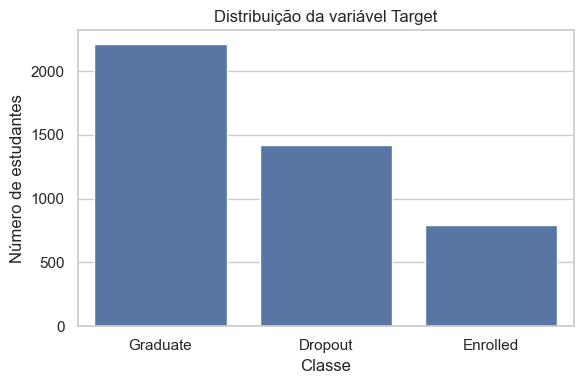
\includegraphics[width=\columnwidth]{figures/notebook_cell_10_01.png}
\caption{Original target distribution. The dataset is dominated by the \textit{Graduate} class (49.93\%), while \textit{Dropout} represents 32.12\% of the records.}
\label{fig:target}
\end{figure}

The data validation step found no missing values and no duplicated rows, which reduced the need for corrective cleaning. The main data-quality limitation is interpretability: many categorical variables are stored as numeric codes, so their meaning depends on external documentation.

The exploratory analysis indicated that academic progression variables are strongly related to the target. Fig.~\ref{fig:academic} shows the distribution of selected academic variables by outcome. Students with fewer approved curricular units and lower grades tend to be more associated with dropout. The correlation heatmap in Fig.~\ref{fig:corr} also suggests dependence between first- and second-semester academic performance indicators. However, this observation must be interpreted carefully: correlation and predictive importance do not prove causality. In addition, several categorical variables are numerically encoded, which limits direct interpretation without external documentation of the category meanings.

\begin{figure}[htbp]
\centering
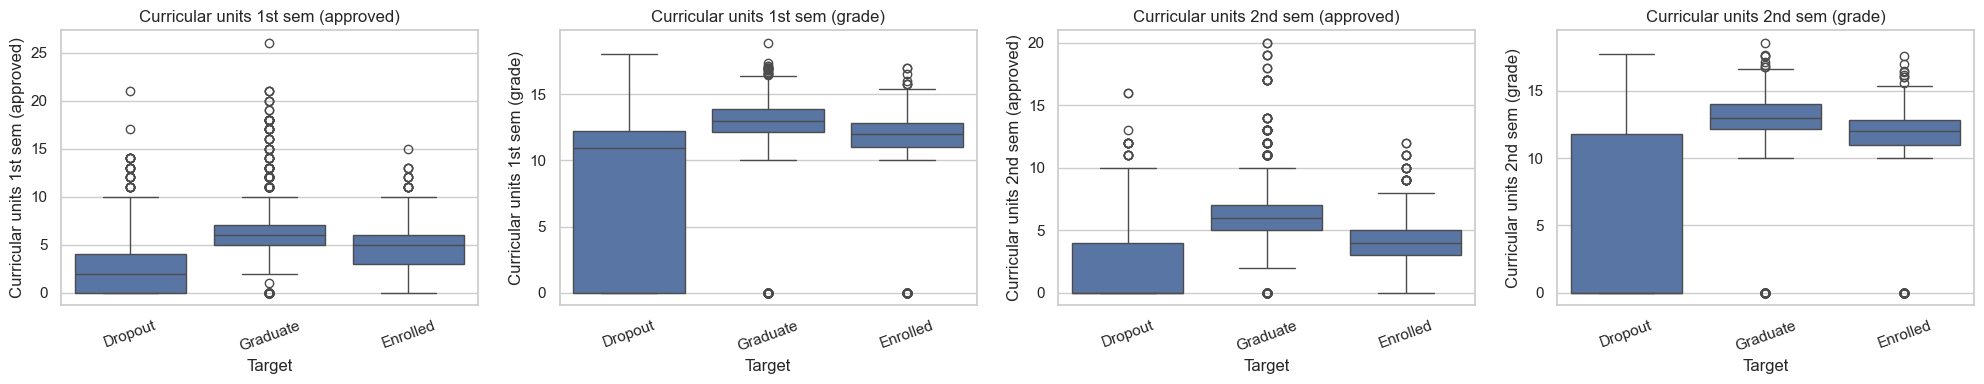
\includegraphics[width=\columnwidth]{figures/notebook_cell_12_00.png}
\caption{Visual exploration of relevant academic variables. Academic progression indicators, especially approved curricular units, show visible separation between target classes.}
\label{fig:academic}
\end{figure}

\begin{figure}[htbp]
\centering
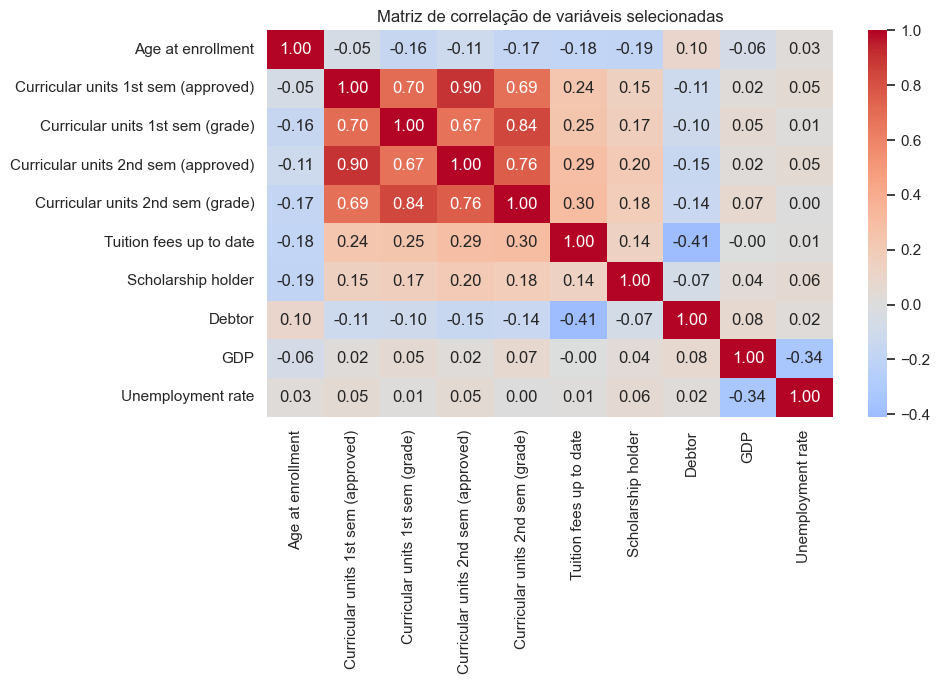
\includegraphics[width=\columnwidth]{figures/notebook_cell_14_00.png}
\caption{Correlation heatmap for selected numerical variables. Several academic variables are correlated, motivating the use of models that can handle interactions and redundancy.}
\label{fig:corr}
\end{figure}

\section{Data Preprocessing}
For the main task, the original target was transformed into a binary variable: students labelled \textit{Dropout} were assigned to the positive class, while \textit{Graduate} and \textit{Enrolled} were grouped as \textit{Non-Dropout}. The data was split into training and test sets using stratification to preserve the class distribution in both partitions. The test set contained 885 students: 284 \textit{Dropout} cases and 601 \textit{Non-Dropout} cases. The training set contained the remaining 3539 students.

The preprocessing and modelling steps were implemented with machine learning pipelines. This is important because transformations are fitted only on the training data inside each validation fold, reducing the risk of data leakage. Numeric features were handled using imputation by the median and standardisation. Categorical features were handled using imputation by the most frequent value and one-hot encoding. Model comparison used 5-fold stratified cross-validation with shuffling and a fixed random seed. Class imbalance was considered during modelling: Logistic Regression, Random Forest and Hist Gradient Boosting used balanced class weights, while AdaBoost and Gradient Boosting were trained with their reported default class weighting. The final comparison relied on F1-score and recall instead of accuracy alone.


\section{Machine Learning Methods}
Several supervised classification algorithms were evaluated. A dummy classifier was included as a baseline, using the most frequent class strategy. Logistic Regression was used as a simple and interpretable linear model, with class weighting to reduce the impact of imbalance. Random Forest was included because it combines multiple decision trees and can model nonlinear interactions. AdaBoost and Gradient Boosting were evaluated as boosting methods that sequentially combine weak learners. Hist Gradient Boosting was also tested as an efficient gradient boosting variant with balanced class weights.

The main Gradient Boosting model used 150 estimators, a learning rate of 0.05 and maximum tree depth of 3. These parameters were the configuration used in the notebook for the final model. The number of estimators controls how many trees are added, the learning rate controls the contribution of each tree and the depth controls the complexity of interactions captured by each tree. The objective during model selection was not only to maximise accuracy but also to obtain a strong F1-score for the dropout class, since both precision and recall matter in a support-oriented early-warning scenario.

\section{Results and Discussion}
Table~\ref{tab:binarycv} and Fig.~\ref{fig:modelcv} summarise the main binary model comparison. The best model according to cross-validated F1-score was Gradient Boosting, with an F1-score of 79.09\% for the target class. Logistic Regression had a very similar F1-score (79.08\%) and higher recall (81.44\%), but lower precision (76.98\%). This difference is important: Logistic Regression would flag more dropout students but also generate more false alarms. Gradient Boosting was selected because it achieved the best F1-score and a stronger precision-recall balance.

\begin{table}[htbp]
\caption{Binary Classification Model Comparison}
\label{tab:binarycv}
\centering
\begin{tabular}{lrrrr}
\toprule
Model & Acc. & F1 & Prec. & Rec. \\
\midrule
Gradient Boosting & 87.62 & 79.09 & 86.57 & 72.82 \\
Logistic Regression & 86.13 & 79.08 & 76.98 & 81.44 \\
Hist Gradient Boosting & 86.63 & 78.99 & 79.82 & 78.19 \\
Random Forest & 86.95 & 77.41 & 87.16 & 69.65 \\
AdaBoost & 85.28 & 75.51 & 81.03 & 70.71 \\
\bottomrule
\end{tabular}
\end{table}

\begin{figure}[htbp]
\centering
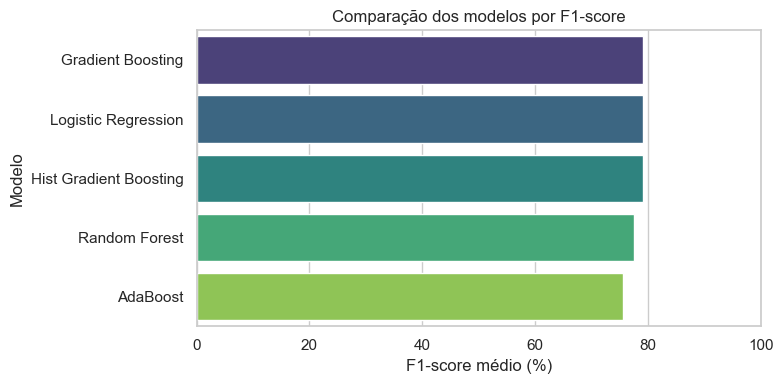
\includegraphics[width=\columnwidth]{figures/notebook_cell_20_03.png}
\caption{Cross-validation comparison of the binary classifiers. Gradient Boosting achieved the best F1-score, while Logistic Regression obtained the highest recall.}
\label{fig:modelcv}
\end{figure}

An additional train-versus-validation diagnostic was used to check for overfitting. For the selected Gradient Boosting model, the training F1-score was 82.64\% and the cross-validated F1-score was 79.09\%, giving a gap of 3.55 percentage points. This difference suggests that the model fits the training data slightly better than unseen validation folds, as expected, but it does not show a strong overfitting pattern. This contrasts with Random Forest and Hist Gradient Boosting, which had larger train-validation gaps of 22.59 and 17.33 percentage points, respectively. Therefore, the selected Gradient Boosting model offered a better compromise between predictive performance and generalisation.

The final test results are shown in Table~\ref{tab:test}. The model achieved 87.57\% accuracy, which indicates good overall predictive performance. However, accuracy alone is not sufficient for this problem because the objective is specifically to detect dropout risk. For the \textit{Dropout} class, the model reached 79.17\% F1-score and 73.59\% recall. The recall value means that approximately one quarter of actual dropout cases were still missed. In an early-warning context, these false negatives are important because they correspond to students who may need support but would not be flagged by the model.

\begin{table}[htbp]
\caption{Final Test Results for Gradient Boosting}
\label{tab:test}
\centering
\begin{tabular}{lr}
\toprule
Metric & Value \\
\midrule
Accuracy & 87.57\% \\
F1-score, Dropout & 79.17\% \\
Recall, Dropout & 73.59\% \\
F1-score, Non-Dropout & 91.14\% \\
\bottomrule
\end{tabular}
\end{table}

\begin{table}[htbp]
\caption{Final Test Confusion Matrix}
\label{tab:confusion}
\centering
\begin{tabular}{lrr}
\toprule
Actual / Predicted & Non-Dropout & Dropout \\
\midrule
Non-Dropout & 566 & 35 \\
Dropout & 75 & 209 \\
\bottomrule
\end{tabular}
\end{table}

\begin{figure}[htbp]
\centering
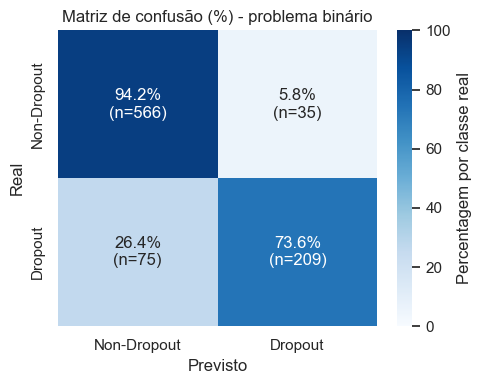
\includegraphics[width=.85\columnwidth]{figures/notebook_cell_22_02.png}
\caption{Confusion matrix for the final Gradient Boosting model. The model correctly identified 209 of 284 dropout students, but missed 75.}
\label{fig:confusion}
\end{figure}

A multiclass experiment was also conducted using the original classes. In that setting, Hist Gradient Boosting achieved the best macro F1-score among the tested models, with 77.08\% accuracy, 71.35\% balanced accuracy and 71.74\% macro F1-score. On the test set, the multiclass model obtained 76.87\% F1-score for \textit{Dropout}, 50.72\% for \textit{Enrolled} and 83.88\% for \textit{Graduate}. The multiclass results were weaker than the binary results, especially for \textit{Enrolled}. This is expected because \textit{Enrolled} is an intermediate state and may represent students whose final academic outcome is not yet fully determined. Compared with the reviewed literature, the obtained binary accuracy of 87.57\% is consistent with the strong performance usually reported for ensemble methods. Direct numerical comparison is limited, however, because studies differ in dataset, country, target definition, validation protocol and the moment in the academic path when features become available.

Model interpretation was performed using permutation importance. As shown in Fig.~\ref{fig:importance}, the most influential variable was \textit{Curricular units 2nd sem (approved)}, with importance 0.2320. The next most relevant feature was \textit{Tuition fees up to date}, with importance 0.0770. The remaining top features had much smaller importance values: \textit{Scholarship holder} (0.0116), \textit{Age at enrollment} (0.0075) and \textit{Curricular units 1st sem (approved)} (0.0070). This difference indicates that second-semester academic progression dominates the prediction. The conclusion is technically useful but also critical: if the purpose is very early intervention, relying on second-semester information may be too late for some institutional actions.

\begin{figure}[htbp]
\centering
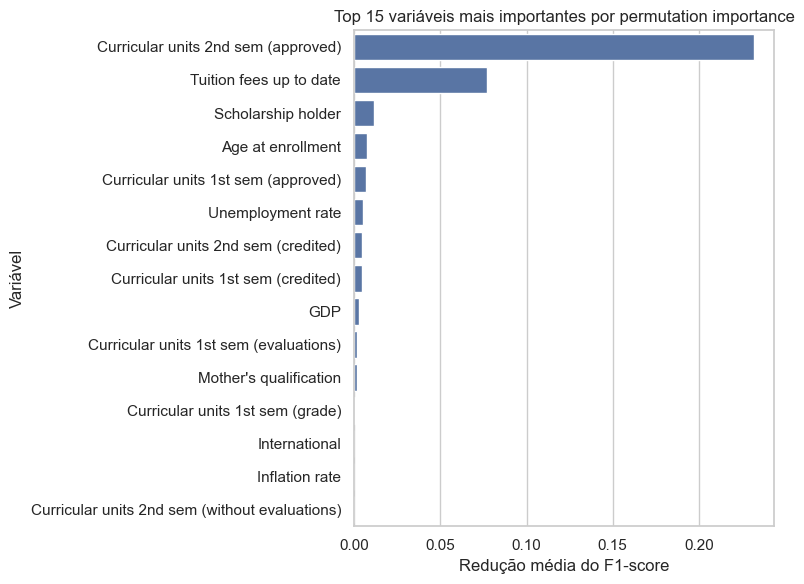
\includegraphics[width=\columnwidth]{figures/notebook_cell_24_02.png}
\caption{Permutation importance for the final Gradient Boosting model. Second-semester approved curricular units dominate the ranking.}
\label{fig:importance}
\end{figure}

These features are plausible from an educational perspective, as academic progression and financial/administrative status are naturally related to dropout risk. Still, importance should not be read as causal evidence. For example, being a scholarship holder or having tuition fees up to date may reflect broader socioeconomic conditions rather than directly causing student success.

An ethical analysis was also considered by evaluating performance across subgroups. The largest observed recall gap occurred for \textit{Tuition fees up to date}: dropout recall was 97.96\% for students without tuition fees up to date and 60.75\% for students with tuition fees up to date, a gap of 37.21 percentage points. Scholarship holder status also showed a relevant gap of 20.51 percentage points, while debtor status showed 18.20 percentage points. Gender showed a much smaller gap of 2.19 percentage points. These numbers do not prove unfairness by themselves, because subgroup sizes and base dropout rates differ, but they show that a deployed system would require continuous monitoring.

\begin{table}[htbp]
\caption{Recall Gap for the Dropout Class by Subgroup}
\label{tab:fairness}
\centering
\begin{tabular}{lrrr}
\toprule
Subgroup & Min & Max & Gap \\
\midrule
Debtor & 70.26 & 88.46 & 18.20 \\
Gender & 72.46 & 74.66 & 2.19 \\
Scholarship holder & 55.17 & 75.69 & 20.51 \\
Tuition fees up to date & 60.75 & 97.96 & 37.21 \\
\bottomrule
\end{tabular}
\end{table}

\section{Conclusions}
This project shows that supervised machine learning can predict student dropout with useful performance on the analysed dataset. Gradient Boosting was the strongest binary model by cross-validated F1-score and achieved 87.57\% test accuracy. More importantly, it detected 209 of the 284 dropout cases in the test set. This means that the model identified approximately 73.59\% of students who actually dropped out. At the same time, it missed 75 dropout students and incorrectly flagged 35 non-dropout students as dropout. These numbers lead to a practical conclusion: the model is useful as a prioritisation tool, but it is not reliable enough to be used as an automatic decision system.

The main advantage of the selected approach is its predictive strength and ability to capture nonlinear relationships. Its main disadvantages are lower interpretability compared with Logistic Regression and the possibility of detecting risk too late if second-semester variables are required. The feature importance analysis supports this concern: the most important variable had importance 0.2320 and corresponds to second-semester approved curricular units. Therefore, a model trained only on enrolment or first-semester data should be evaluated in future work, even if its accuracy decreases, because it may be more useful for early intervention.

\section{Future Work}
Future work should first include a more systematic hyperparameter optimisation process. In this project, Gradient Boosting used 150 estimators, a learning rate of 0.05 and maximum depth of 3. A wider search over the number of estimators, learning rate, tree depth and regularisation parameters could improve the current test results of 87.57\% accuracy and 79.17\% F1-score for \textit{Dropout}. This search should also compare training and validation performance to identify possible overfitting or underfitting more rigorously than the simple diagnostic used in this work.

A second direction is to improve the treatment of class imbalance and increase recall for the dropout class. The final Gradient Boosting model obtained 73.59\% recall for \textit{Dropout}, meaning that 75 of the 284 dropout students in the test set were missed. Since Logistic Regression reached 81.44\% recall in cross-validation, compared with 72.82\% for Gradient Boosting, future experiments should explicitly study models or settings that detect more at-risk students. Possible improvements include tuning the decision threshold, comparing class weighting across all models and testing oversampling methods such as SMOTE inside the cross-validation pipeline.

A third improvement is to evaluate threshold-independent metrics and probability quality. The current report focuses on accuracy, F1-score, precision and recall at the default decision threshold. Future work should add ROC curves, Precision-Recall curves, AUROC and Average Precision to analyse model behaviour across all thresholds, especially because the positive class is the minority class. Probability calibration should also be evaluated using methods such as Platt scaling or isotonic regression, because in a real early-warning system counsellors may interpret the model output as a risk score rather than only as a binary label.

A fourth improvement is to analyse the moment at which variables become available. The current best model relies strongly on \textit{Curricular units 2nd sem (approved)}, whose permutation importance was 0.2320. This makes the model accurate but potentially late for early intervention. A future version should compare enrolment-only features, first-semester features and the full feature set, making explicit the trade-off between earlier prediction and predictive performance.

Finally, future work should deepen interpretability, fairness and deployment validation. SHAP values or partial dependence plots could explain individual predictions more clearly than global permutation importance, while also helping to check whether correlated academic variables share importance. Fairness should also be monitored because the observed recall gap reached 37.21 percentage points for tuition-fee status and 20.51 percentage points for scholarship holder status. Before real deployment, the model should be validated with data from other academic years or institutions to test whether performance remains stable under possible distribution shift.

\section{Critical Reflection}
This work reinforced that building a machine learning model is not only a technical exercise. The choice of target, evaluation metric and validation method changes the meaning of the results. In this project, optimising only accuracy would be insufficient because missing a dropout student may be more serious than incorrectly flagging a student who is not at risk. The final accuracy was 87.57\%, but the dropout recall was 73.59\%; this difference shows why class-specific metrics are necessary. The project also made clear the importance of avoiding data leakage through pipelines and stratified validation. Without these precautions, performance estimates could look better than they really are.

Another important lesson is that model performance must be interpreted in context. A high score on a historical dataset does not guarantee that the model will generalise to future cohorts or other institutions. The analysis also showed that strong predictive variables can be sensitive: financial and academic indicators may help prediction, but they must be used responsibly. Therefore, the most responsible use of this type of model is as an early-warning support tool combined with human judgement, continuous evaluation and clear ethical rules.

\section{AI Tools}
OpenAI Codex/ChatGPT was used to support the organisation of the notebook, improve the structure of the report, suggest future work directions and assist with technical writing because it allowed fast iteration over code, LaTeX structure and result explanation. Claude was also used to discuss ideas and support the formulation of conclusions from the obtained results, especially the interpretation of limitations and ethical implications. The modelling decisions, interpretation of results and final responsibility for the submitted work remain with the students. AI assistance was used as a drafting and review aid, not as a substitute for understanding or validating the project.

\begin{thebibliography}{00}
\balance

\bibitem{kovacic2010early}
Z. Kovacic, ``Early prediction of student success: Mining students enrolment data,'' \textit{Proceedings of Informing Science \& IT Education Conference}, pp. 647--665, 2010.

\bibitem{ames2016dropout}
A. Aulck, N. Velagapudi, J. Blumenstock and J. West, ``Predicting student dropout in higher education,'' \textit{arXiv preprint arXiv:1606.06364}, 2016.

\bibitem{nagy2018predicting}
M. Nagy and R. Molontay, ``Predicting dropout in higher education based on secondary school performance,'' in \textit{Proc. IEEE 22nd International Conference on Intelligent Engineering Systems}, 2018, pp. 389--394.

\bibitem{miguéis2018early}
V. L. Migueis, A. Freitas, P. J. V. Garcia and A. Silva, ``Early segmentation of students according to their academic performance: A predictive modelling approach,'' \textit{Decision Support Systems}, vol. 115, pp. 36--51, 2018.

\bibitem{lee2023study}
S. Lee and J. Chung, ``A study on dropout prediction for university students using machine learning,'' \textit{Applied Sciences}, vol. 13, no. 21, 2023.

\bibitem{martinho2023supervised}
V. Martinho, C. Nunes and C. Minussi, ``Supervised machine learning algorithms for predicting student dropout and academic success: A comparative study,'' \textit{Discover Artificial Intelligence}, vol. 3, 2023.

\bibitem{uci2021dropout}
UCI Machine Learning Repository, ``Predict Students' Dropout and Academic Success,'' 2021. [Online]. Available: \url{https://archive.ics.uci.edu/dataset/697/predict+students+dropout+and+academic+success}

\bibitem{oecd2025completion}
OECD, ``Who is expected to complete tertiary education?,'' in \textit{Education at a Glance 2025}, OECD Publishing, 2025. [Online]. Available: \url{https://www.oecd.org/en/publications/education-at-a-glance-2025_1c0d9c79-en/full-report/who-is-expected-to-complete-tertiary-education_a1099e2e}

\bibitem{ec2025monitor}
European Commission, ``Education and Training Monitor 2025: Comparative report,'' 2025. [Online]. Available: \url{https://op.europa.eu/webpub/eac/education-and-training-monitor/en/comparative-report/chapter-6.html}

\bibitem{eurostat2025dropout}
Eurostat, ``14\% of young people in the EU dropped out of education,'' 2025. [Online]. Available: \url{https://ec.europa.eu/eurostat/web/products-eurostat-news/w/ddn-20251215-3}

\bibitem{github2026project}
G. Simões, H. Reveles and G. Santos, ``iaa-project-1,'' GitHub repository, 2026. [Online]. Available: \url{https://github.com/goncaloosimoes/iaa-project-1}

\end{thebibliography}

\end{document}
